\section{ONIWALDUS BERE MALI (1174005)}
\subsection{Pengertian}
Sistem Informasi Geografis (SIG) atau Geographic Information System (GIS) adalah sustem informai khusu yang mengelola data yang memiliki informasi spasial yaitu bereferensi keruangan. Atau lebih singkatnya, sistem informasi geografis adalah h sistem komputer yang mempunyai kemampuan untuk membangun, menyimpan, mengelola dan menampilkan informasi berefrensi geografis, misalnya data diidentifikasi menurut lokasinya dalam sebuah database.
Teknologi Sistem Informasi Geografis digunakan untuk investigasi ilmiah, pengelolaan sumber daya, perencanaan pembangunan, kartografi dan perencanaan rute. Contohnya SIG dapat digunakan perencana untuk membantu menghitung waktu tanggap darurat saat terjadi bencana alam secara cepat dan lain sebagainya.

\subsection{Sejarah}
35000 tahun yang lalu, di dinding gua Lascaux, Perancis, para pemburu Cro-Magnon menggambar hewan mangsa mereka, dan juga garis yang dipercaya sebagai rute migrasi hewan-hewan tersebut. Catatan awal ini sejalan dengan dua elemen struktur pada sistem informasi gegrafis modern sekarang ini, arsip grafis yang terhubung ke database atribut.
Pada tahun 1700-an teknik survey modern untuk pemetaan topografis diterapkan, termasuk juga versi awal pemetaan tematis, misalnya untuk keilmuan atau data sensus.
Awal abad ke-20 memperlihatkan pengembangan “litografi foto” dimana peta dipisahkan menjadi beberapa lapisan (layer). Perkembangan perangkat keras komputer yang dipacu oleh penelitian senjata nuklir membawa aplikasi pemetaan menjadi multifungsi pada awal tahun 1960-an.
Tahun 1967 merupakan awal pengembangan SIG yang bisa diterapkan di Ottawa, Ontario oleh Departemen Energi, Pertambangan dan Sumber Daya. Dikembangkan oleh Roger Tomlinson, yang kemudian disebut CGIS (Canadian GIS – SIG Kanada), digunakan untuk menyimpan, menganalisis dan mengolah data yang dikumpulkan untuk Inventarisasi Tanah Kanada (CLI – Canadian land Inventory) – sebuah inisiatif untuk mengetahui kemampuan lahan di wilayah pedesaan Kanada dengan memetakaan berbagai informasi pada tanah, pertanian, pariwisata, alam bebas, unggas dan penggunaan tanah pada skala 1:250000. Faktor pemeringkatan klasifikasi juga diterapkan untuk keperluan analisis.
GIS dengan gvSIG.
CGIS merupakan sistem pertama di dunia dan hasil dari perbaikan aplikasi pemetaan yang memiliki kemampuan timpang susun (overlay), penghitungan, pendijitalan/pemindaian (digitizing/scanning), mendukung sistem koordinat national yang membentang di atas benua Amerika , memasukkan garis sebagai arc yang memiliki topologi dan menyimpan atribut dan informasi lokasional pada berkas terpisah. Pengembangya, seorang geografer bernama Roger Tomlinson kemudian disebut “Bapak SIG”.

\subsection{Koordinat}
Penginderaan Jauh
Penginderaan jauh adalah metode pengambilan informasi dan pencatatan rupabumi suatu wilayah dengan menggunakan wahana tertentu.Sesuai dengan namanya, surveyor yang menggunakan penginderaan jauh umumnya berlokasi jauh atau tidak langsung berada di wilayah survey. Hal ini dapat terjadi karena kemajuan teknologi pada bidang foto udara, sensor, pesawat, serta satelit.Penginderaan jauh umumnya dilakukan dengan menggunakan foto udara dari pesawat, foto satelit, atau teknologi drone.
GPS atau Global Positioning System adalah sistem penentuan lokasi global yang memanfaatkan satelit untuk melakukan triangulasi lokasi perangkat.
Global positioning system berkerja dengan cara menerima sinyal dari satelit yang nantinya akan digunakan untuk melakukan triangulasi lokasi. Oleh karena itu, GPS hanya dapat berfungsi secara akurat jika terdapat 3 atau lebih satelit yang mengirimkan sinyal.
Selain itu, GPS juga harus memiliki koneksi sinyal yang bagus dengan satelit tersebut agar dapat memprediksi lokasi secara akurat.Sekarang, GPS sudah memiliki akurasi dibawah 10m sehingga mengurangi galat saat melakukan perhitungan atau navigasi. GPS navigais tertentu bahkan sudah mencapai akurasi dibawah 3-5m, sedangkan GPS untuk survei dan pemetaan sudah memiliki akurasi dalam rentang milimeter.Meskipun begitu, perangkat GPS yang memiliki kualitas dan akurasi tinggi sangat sulit didapatkan dan memiliki harga yang mahal. Oleh karena itu, tidak semua orang dapat mengakses sebuah GPS.Sistem informasi geografis memiliki banyak manfaat, 
Koordinat adalah suatu titik yang didapatkan dari hasil perpotongan dari garis latitude (lintang) dengan garis bujur (longitude) sehingga akan menunjukan lokasi pada suatu daerah. Umumnya koordinat dibedakan menjadi koordinat Geographic dan Universal Transver Mercator (UTM). Pada Koordinat Geogprahic dibedakan menjadi tiga berdasarkan satuannya yaitu :
1.	Degree, Decimal (DD,DDDD) Contoh : S 3.56734 E 104.67235
2.	Degree, Minute (DD MM,MMMM) Contoh : S 3⁰ 43,5423’ E 104 33,6445’
3.	Degree, Minute, Second (DD MM SS,SS) Contoh : S 3⁰ 43’ 45,22” E104 33’ 33,25”
Pada Bujur/Longitude (X) merupakan garis yang perpindahannya secara vertical dan pada Lintang/Lattitude (Y) merupakan garis yang mempunyai perpindahan secara horizontal, pada (Gambar 1) menjelaskan perpotongan antara garis bujur dan garis lintang akan membentuk suatu titik pertemuan yang biasa disebut dengan titik koordinat. Pada Sistem Koordinat UTM biasanya terdapat pembagian waktu berdasarkan zonasinya, di Indonesia sendiri terdapat 16 pembagian zonasi waktu, pada Gambar 2 menjelaskan pembagian zonasi waktu dimana terdapat garis yang memisahkan dari garis khatulistiwa. Untuk Daerah yang berada di atas garis khatulistiwa akan mempunyai Kode N sedangkan yang berada dibawah khatulistiwa akan mempunyai kode S.Saat penggunaan GPS biasanya terdapat pengaturan untuk melakukan konversi pada satuan koordinat sehingga memudahkan pengguna berdasarkan kebutuhan yang diinginkan. Konversi pun dapat dilakukan dengan merubah satuan Koordinat Geografis DD MM SS,SS menjadi DD,DDDD ataupun sebaliknya.

\subsection{Data Geospasial}
Data geospasial adalah kumpulan fakta yang berupa informasi tentang ruang kebumian (geospasial) yang menunjukan lokasi atau posisi dari suatu tempat atau objek yang direpresentasikan pada sebuah garis titik koordinat. Data geospasial dibagi menjadi 2 yaitu:
Data Vector
Dalam bentuk data vector bagian objek dibumi ditampilkan sebagai kumpulan titik , garis dan polygon dimana sekumpulan tiitik yang saling terhubung akan membentuk garis dan garis yang saling terhubung antara titik awal dan titik akhir dengan nilai koordinat ynag sama akan membentuk polygon . Data vector dibagi menjadi 2 yaitu :
Culture
Culture memaparkan atau menampilkan data geospasial yang disertai dengan nama atribut atau memberikan keterangan atas nama dari objek di bumi. Contohnya nama dari suatu Negara, indicator batas air (keterangan kedalaman air laut), nama provinsi, daerah, wilayah dsb.
populated-culture
Physical
Physical memaparkan atau menampilkan data geospasial mengenai bentuk fisiknya atau gambaran tentang objek-objek alam yang ada dibumi.
2. Data Raster
Data raster menampilkan permukaan bumi seperti bentuk aslinya atau seperti dalam peta asli yang terlihat jelas dari setiap objek dengan keadaan alamnya. Data raster dibentuk atau menampilkan objek berupa elemen matriks atau grid , data raster digunakan untuk merepresentasikan objek dari data geospasial mengenai batas-batas yang berubah, ketinggian tanah

\subsection{Link}
\href{https://youtu.be/GYiF4K6OzEg}{klik disini}

\subsection{Plagiarism}
\begin{figure}[H]
	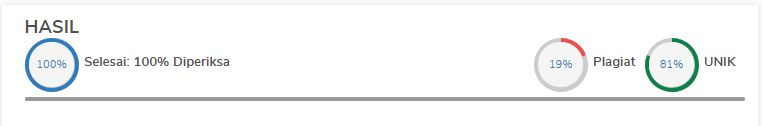
\includegraphics[width=4cm]{figures/1174005/ONI.JPG}
	\centering
	\caption{Gambar plagiat tugas 1}
\end{figure}
